\documentclass[apacite,draftfirst,man]{apa6}
\usepackage{amsmath}
\usepackage{float}
\usepackage{graphicx}
\usepackage{mathrsfs}

\title{Estimation of Feedback Contingency Depends on Executive Function}
\shorttitle{Executive Feedback Contingency}

\threeauthors {Matthew J. Crossley} {W. Todd Maddox} {F. Gregory Ashby}
\threeaffiliations {SRI International}
{Cognitive Design and Statistical Consulting, Austin, Texas}
{University of California, Santa Barbara}


\abstract{Individuals in drug rehabilitation often experience relapse when
returned to the original context of their drug use. Why do treatments generalize
so poorly across different contexts? We recently addressed this question in the
domain of procedural learning, which is thought to play an important role in
forms of addiction, bad habits, and other maladaptive states
\cite{crossley_erasing_2013}. Our work suggests that feedback contingency,
defined as the correlation between response confidence and outcome, plays a
vital role in controlling a gate that normally prevents procedural knowledge
from being modified during interventions. In particular, our results suggested
that modification of procedural knowledge is possible only if feedback
contingency is high. Here, we ask whether the estimation of feedback contingency
depends on executive mechanisms (e.g., prefrontal networks involved in working
memory and executive reasoning). Our rationale is as follows: If the estimation
of feedback contingency requires executive function, then increasing cognitive
load during intervention via the concurrent performance of an additional task
should disrupt the accurate estimation of contingency, thereby keeping the gate
on procedural learning open. We report the results from an experiment following
this logic that suggests that feedback contingency estimation is indeed
supported by executive function.}

\rightheader{Dual-Task Unlearning} \leftheader{Dual-Task Unlearning}

\begin{document}
\maketitle

\section*{Introduction}
Relapse often occurs when an addict returns to the original context of their
drug use \cite{higgins_outpatient_1995}. This may occur because interventions
given in clinics do not modify addiction-driving stimulus-response (SR)
associations, but instead cause the learning of new clinic-specific
associations. Returning to the original context of drug abuse then reactivates
the preserved addiction-driving SR associations, causing relapse. If true, then
this hypothesis means that the brain has a gating mechanism to protect learning
obtained in old contexts from being modified. Our prior work, which was focused
on understanding this gating mechanism \cite{crossley_erasing_2013}, found that
feedback contingency -- defined as the correlation between response confidence
and outcome -- is a principle driver of this gate. The present study is an
extension of this earlier work, asking whether the estimation of feedback
contingency depends on executive mechanisms. The rest of the introduction
proceeds with a brief summary of the key findings reported by
\cite{crossley_erasing_2013}, followed by the logic of the current study.

\subsection*{Crossley et al. (2013)}
\citeA{crossley_erasing_2013} attempted to understand why the SR associations
underlying procedural learning, habits, and addiction are so remarkably
resistant to modification. We developed a task that, after initial acquisition
of SR associations, attempted to erase the just-formed engram. The results
showed promising initial signs of true memory erasure.

Our experiments included three phases of equal duration: acquisition,
intervention, and test. During acquisition, all participants were trained on the
II categories shown in panel C of Figure \ref{fig:test_cats}. During
intervention, the category structure was unchanged, but feedback about response
accuracy was manipulated in an attempt to erase the learning that occurred
during the initial acquisition. Our goal was to erase the initially acquired SR
associations by overwriting them with random associations.

We investigated the effects of three different types of intervention. All used
random feedback (RF) on some percentage of intervention trials. In the RF(.25)
conditions, the intervention feedback was random on all trials. Since there are
four categories, every intervention response was followed by positive feedback
with probability .25 and negative feedback with probability .75. In the RF(.40)
conditions, RF was also given on every trial, but the probability of positive
feedback was .40 and the probability of negative feedback was .60. Finally, in
the mixed feedback conditions, RF was given with probability .75 and true
feedback was given with probability .25.

In all conditions, feedback returned to 100\% veridical during the test phase.
Half the participants in each condition relearned the original categories (the
relearning conditions) and half learned new categories that used the same
stimuli but permuted the category-response mappings. Thus the study included six
conditions created from a 3 $\times$ 2 factorial design where three levels of
intervention feedback [RF(.25), RF(.40), mixed feedback] were crossed with two
levels of test (relearning, new learning).

\begin{figure}[t]
\centering 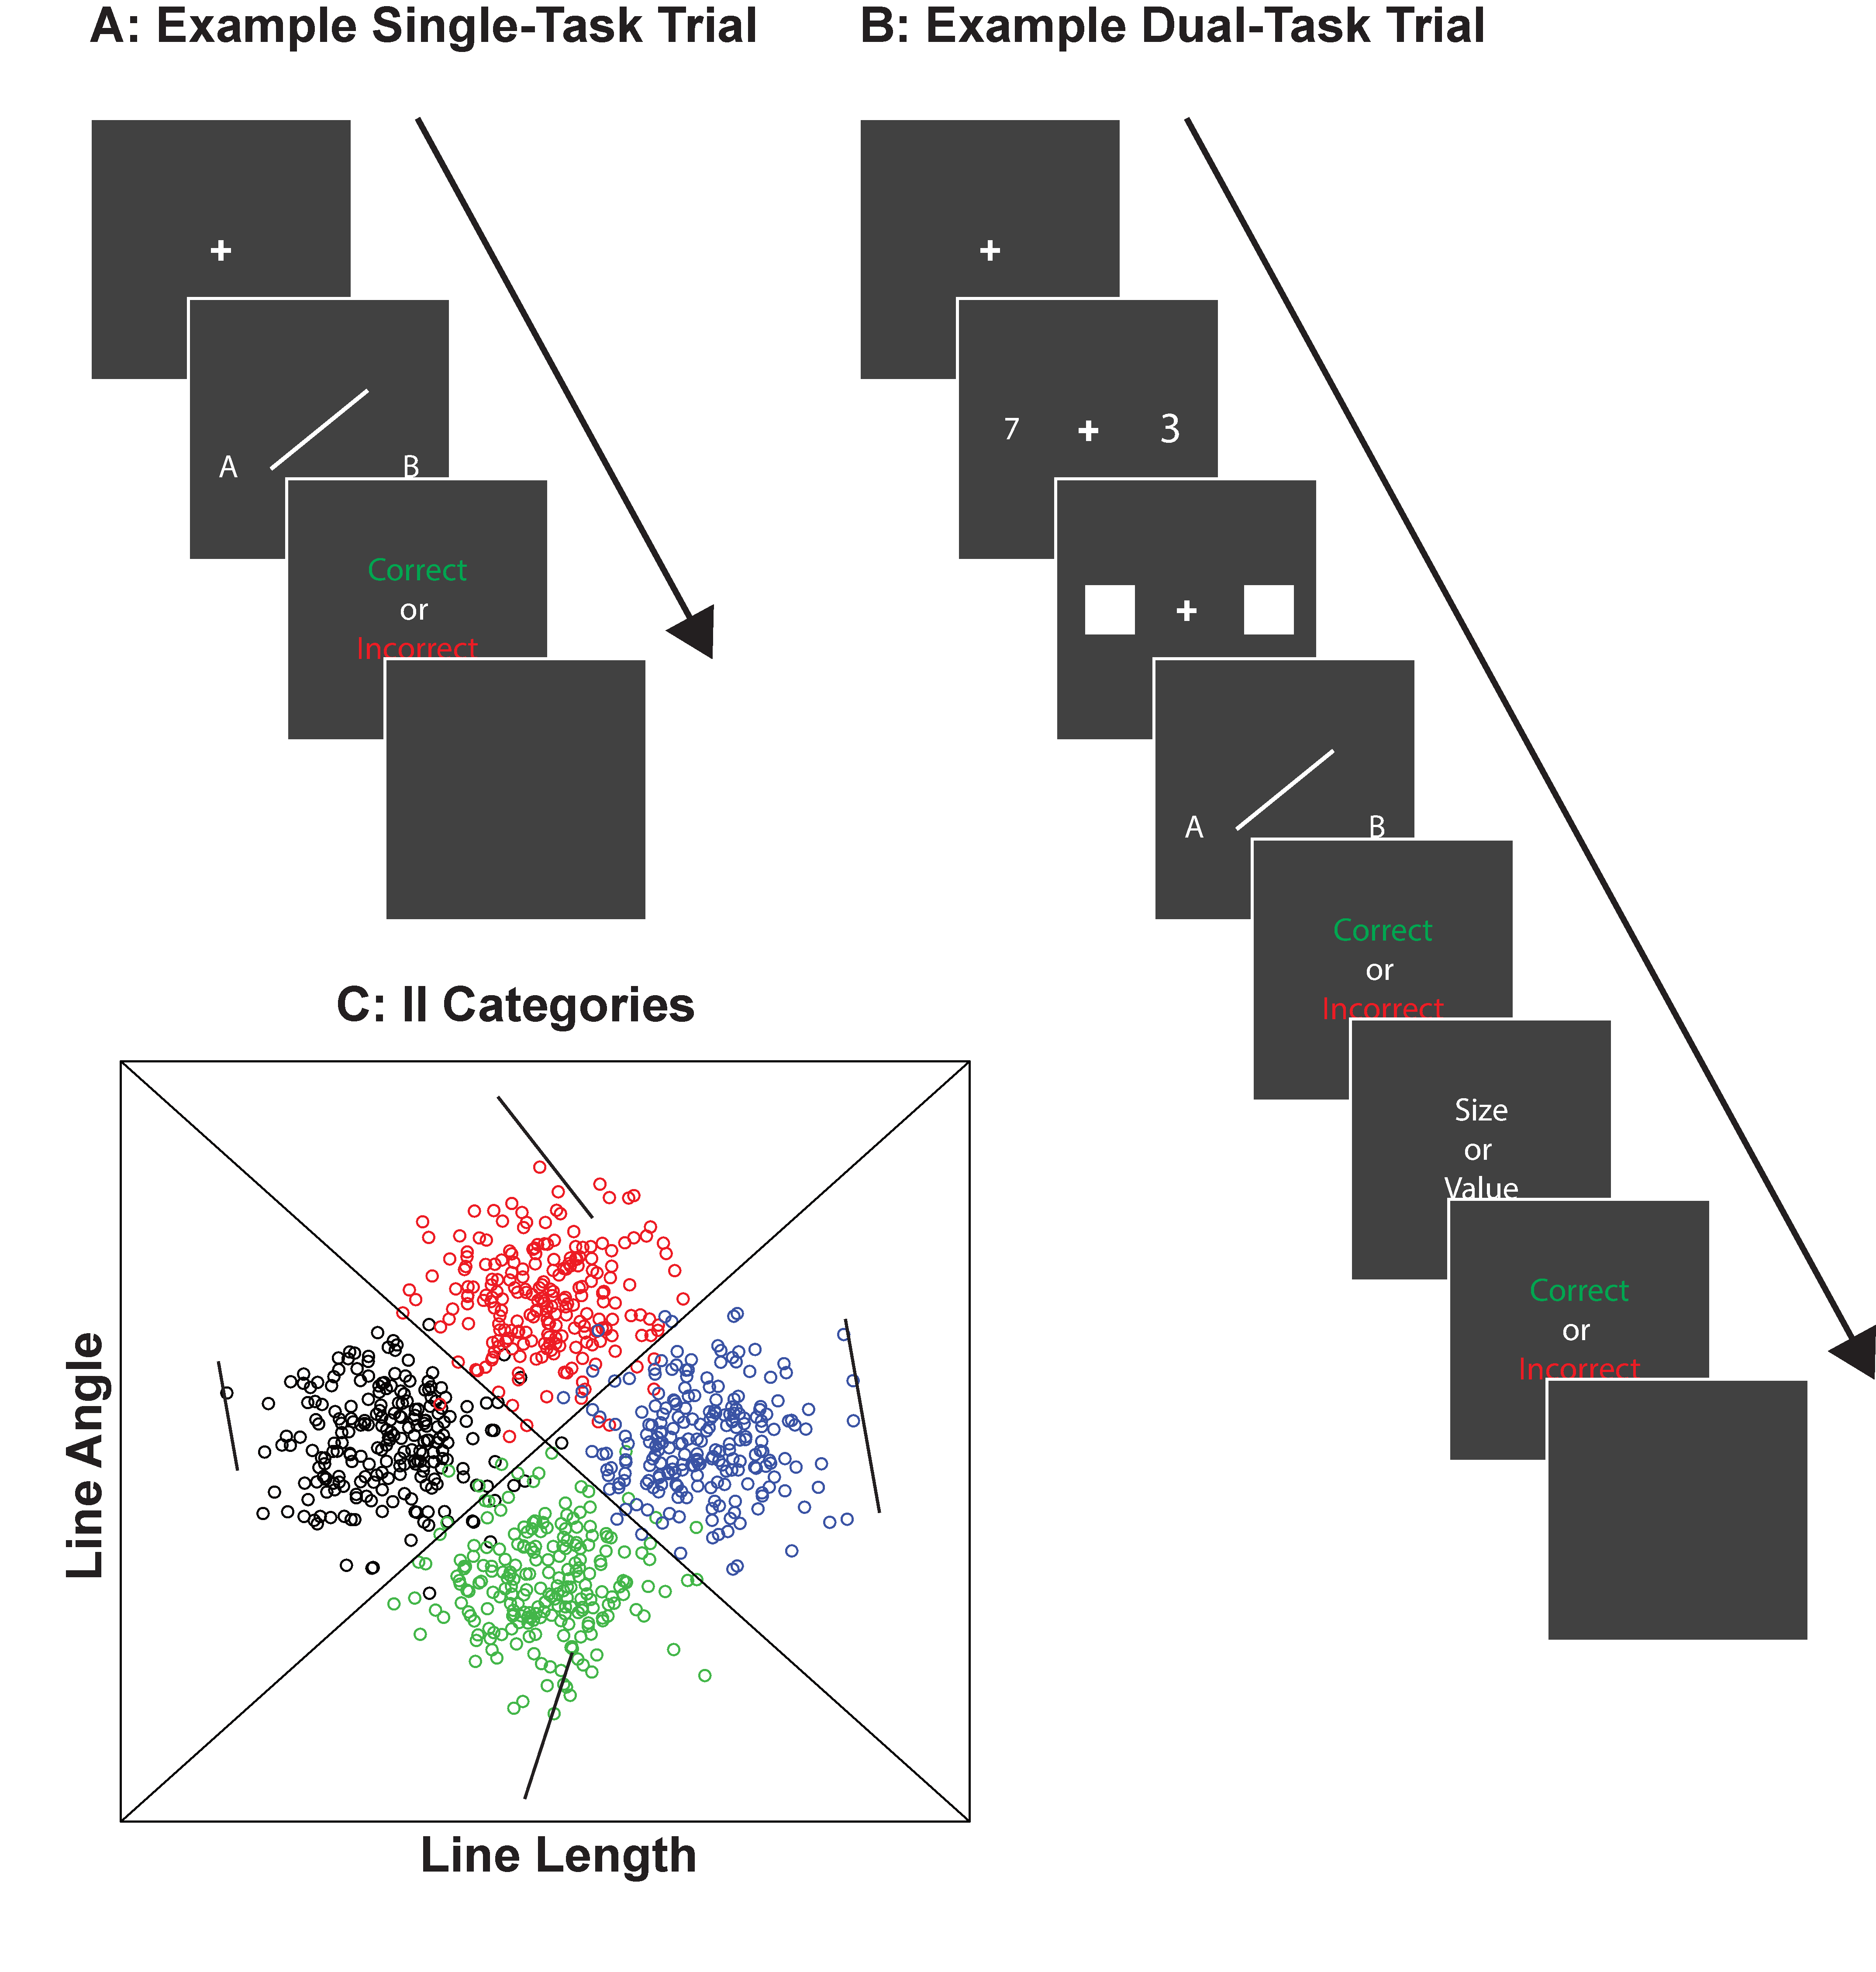
\includegraphics[width=1.0\textwidth]{../figures/fig_trials.pdf}
  \caption{ \textbf{A:} An Example trial during single-task conditions.
\textbf{B:} An example trial during dual-task conditions. \textbf{C:} The II
categories used during the acquisition phase of Crossley et al. (2013). }
  \label{fig:test_cats}
\end{figure}

Operationally, we require two conditions to conclude that unlearning is
successful: (1) the behavior disappears during the intervention, (2) during
test, both relearning and new learning occur at the same rate as initial
learning. In contrast, if learning is preserved during the intervention, then
relearning the original categories should be faster than initial acquisition and
learning of new categories should be slower (because of interference).

Results are shown in Fig. \ref{fig:unlearning_data}. In the RF conditions (Fig.
\ref{fig:unlearning_data}A and \ref{fig:unlearning_data}C), reacquisition is
faster than initial learning, and new category learning is slower, suggesting
that RF does not cause unlearning. In contrast, following mixed feedback
intervention, reacquisition and new category learning both occur at
approximately the same rate as initial learning. Thus, this intervention may
have caused true unlearning.

The RF results are incompatible with classic models (see Figure
\ref{fig:models}A), which assume that procedural skills are learned at
cortical-striatal synapses via DA-dependent synaptic plasticity, and that the DA
signal is proportional to the reward prediction error (RPE = Obtained Reward --
Predicted Reward). Since RF is by definition unpredictable, it generates large
RPEs, and therefore classic models predict that RF will cause new learning of
random associations, which will overwrite the original category knowledge,
causing true unlearning. In contrast, Figure \ref{fig:unlearning_data}A and
\ref{fig:unlearning_data}C show that RF did not disrupt the previously acquired
category knowledge.

\begin{figure}[h]
\centering 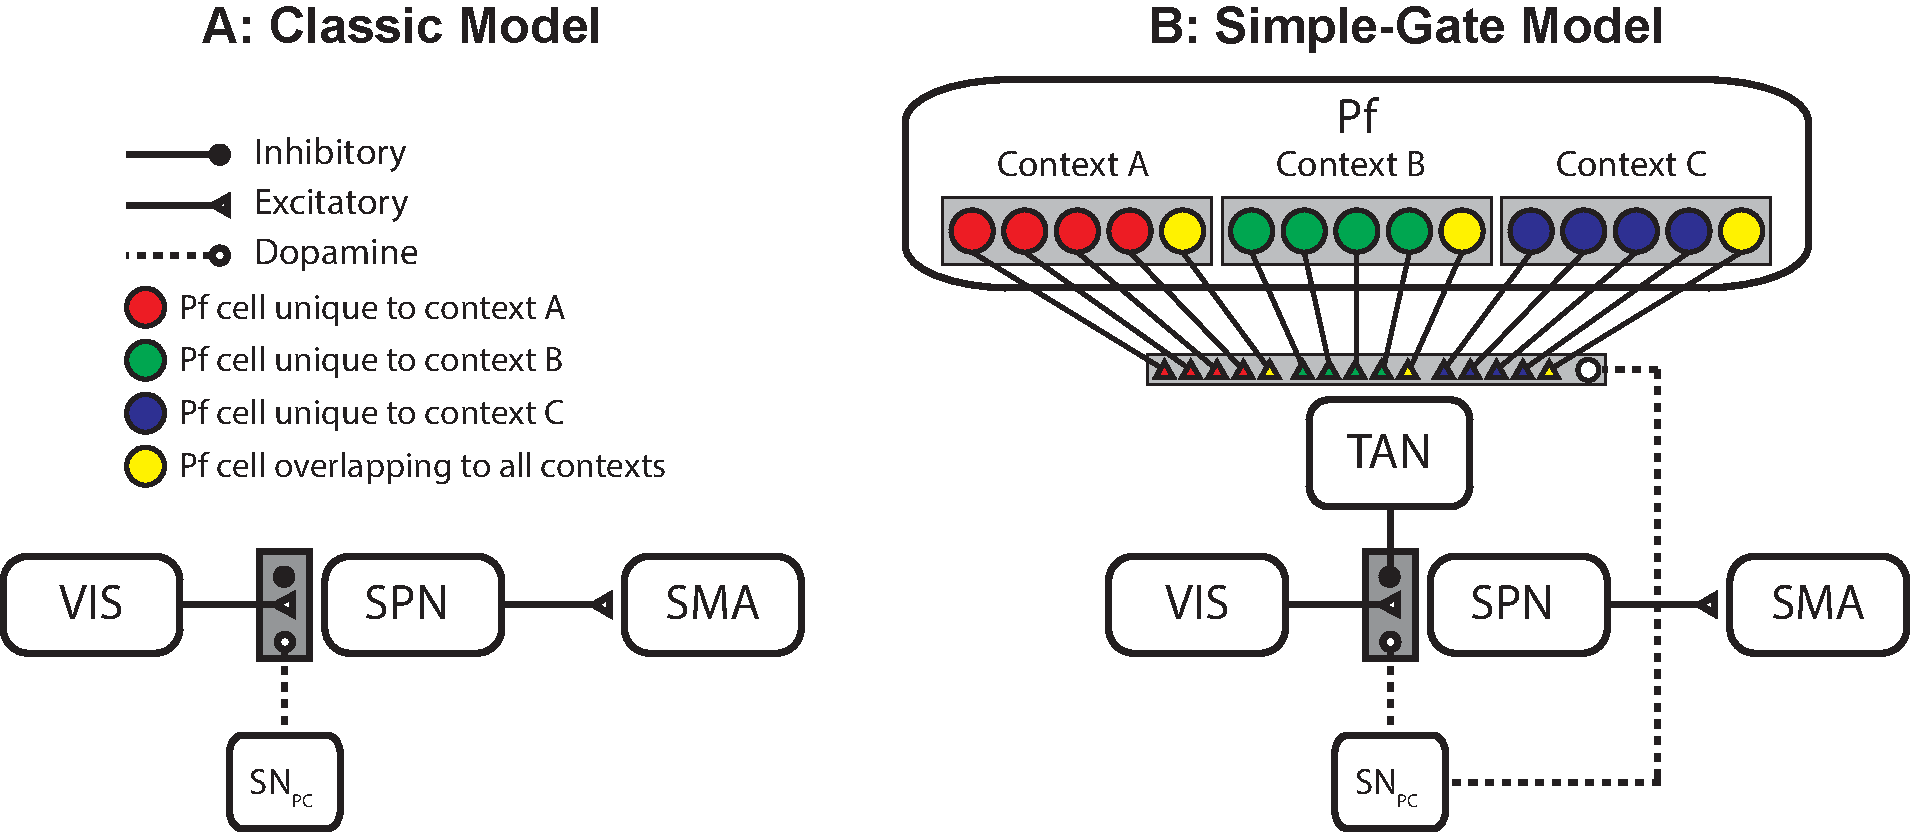
\includegraphics[width=1.0\textwidth]{../figures/fig_models.pdf}
\caption{ \textbf{A: The Classic Model.} A classic model of procedural
  learning based on a greatly simplified representation of the ``direct pathway''
  through the basal ganglia. S-R associations are learned at cortical-striatal
  synapses, which are modified via dopamine-dependent reinforcement learning. The
  likelihood of repeating actions that lead to \emph{unexpected} positive outcomes
  is gradually increased, and the likelihood of repeating actions that lead to
  \emph{unexpected} negative outcomes is gradually decreased. \textbf{B: The TANs
    Model.} The classic model of procedural learning with the addition of a
  context-specific Pf-TAN pathway. This pathway acts as a gate on
  cortical-striatal synaptic plasticity, permitting or preventing the learning and
  expression of procedural knowledge. (SPN - spiny projection neuron of the
  striatum. D1 - Direct pathway SPN expressing the D1 DA receptor. D2 - Indirect
  pathway SPN expressing the D2 DA receptor. SMA - Supplementary Motor Area. SNpc
  - substantia nigra pars compacta. Pf - parafascicular nucleus of the thalamus.
  VIS - visual cortex)}
  \label{fig:models}
\end{figure}

Rapid relearning following RF suggests that \textbf{a gating mechanism protects
procedural knowledge during RF.} We proposed striatal cholinergic interneurons
called TANs (Tonically Active Neurons) as a candidate gate
\cite{AshbyCrossley2011, crossley_erasing_2013}. In their default state, TANs
exert a tonic presynaptic inhibition of cortical inputs to the striatum (Figure
\ref{fig:models}) \cite{calabresi_acetylcholine-mediated_2000}. Thus, the
default state of the gate is closed. However, TANs learn to pause in response to
stimuli that predict reward \cite{kimura1984tonically}, removing the presynaptic
inhibition, and allowing striatal neurons to respond to cortical input and
cortical-striatal learning to occur (i.e., the gate opens). The TANs are driven
by centremedian and parafascicular (CM-Pf) intralaminar thalamic nuclei, which
signal salient environmental cues and changes in context \cite{shimo_role_2001,
yamada_tonically_2004, apicella_responses_1997, ravel2006influence}. The TAN
pause occurs only when the CM-Pf--TAN synapse is strong, and learning at both
CM-Pf--TAN and cortical-striatal synapses is driven by DA-mediated reinforcement
signals \cite{suzuki2001dopamine,setyono1982effect}.

Our model that includes the TAN gating mechanism accounts for a variety of
behavioral and physiological data from simple instrumental conditioning tasks
\cite{AshbyCrossley2011, CrossleyEtAl2016}, including rapid relearning following
extinction. However, even this model failed to account for our RF results (Figure
\ref{fig:unlearning_data}A and \ref{fig:unlearning_data}C). This is because we
still modeled DA release as strictly proportional to RPE, which fluctuates
widely during RF. This leads to random fluctuations in the CM-Pf--TAN synaptic
weight, preventing the TANs from reliably closing the gate.

For the TANs to close the gate and protect cortical-striatal plasticity during
RF, two conditions must be met: (1) The model must detect RF. Since RF is
non-contingent on behavior, the valence of feedback earned after each response
is uncorrelated with the confidence that the response was correct (called
\textit{response confidence}). Contrast this with veridical feedback, in which
negative feedback is typically accompanied by low response confidence. We
recently showed that both RB and II learning are exquisitely sensitive to this
feedback contingency \cite{AshbyVucovich2016}. (2) The TANs must close the gate
when RF is detected. This only occurs when CM-Pf--TAN synapses undergo
consistent weakening. \citeA{crossley_erasing_2013} modeled this by assuming
that the DA response is attenuated and biased below baseline when feedback
contingency is low.

With these modifications, the model not only accounts for savings in relearning
after RF intervention, but also makes a novel prediction: \textbf{If true
feedback is given on a small percentage of trials (e.g., 25\%), then the
correlation between feedback valence and response confidence could be high
enough to cause the TANs to pause, allowing the RF on the other (75\%) trials to
induce true unlearning.} Results from our Mixed Feedback intervention (Figure
\ref{fig:unlearning_data}B) are consistent with this prediction.

\begin{figure}[h]
\centering 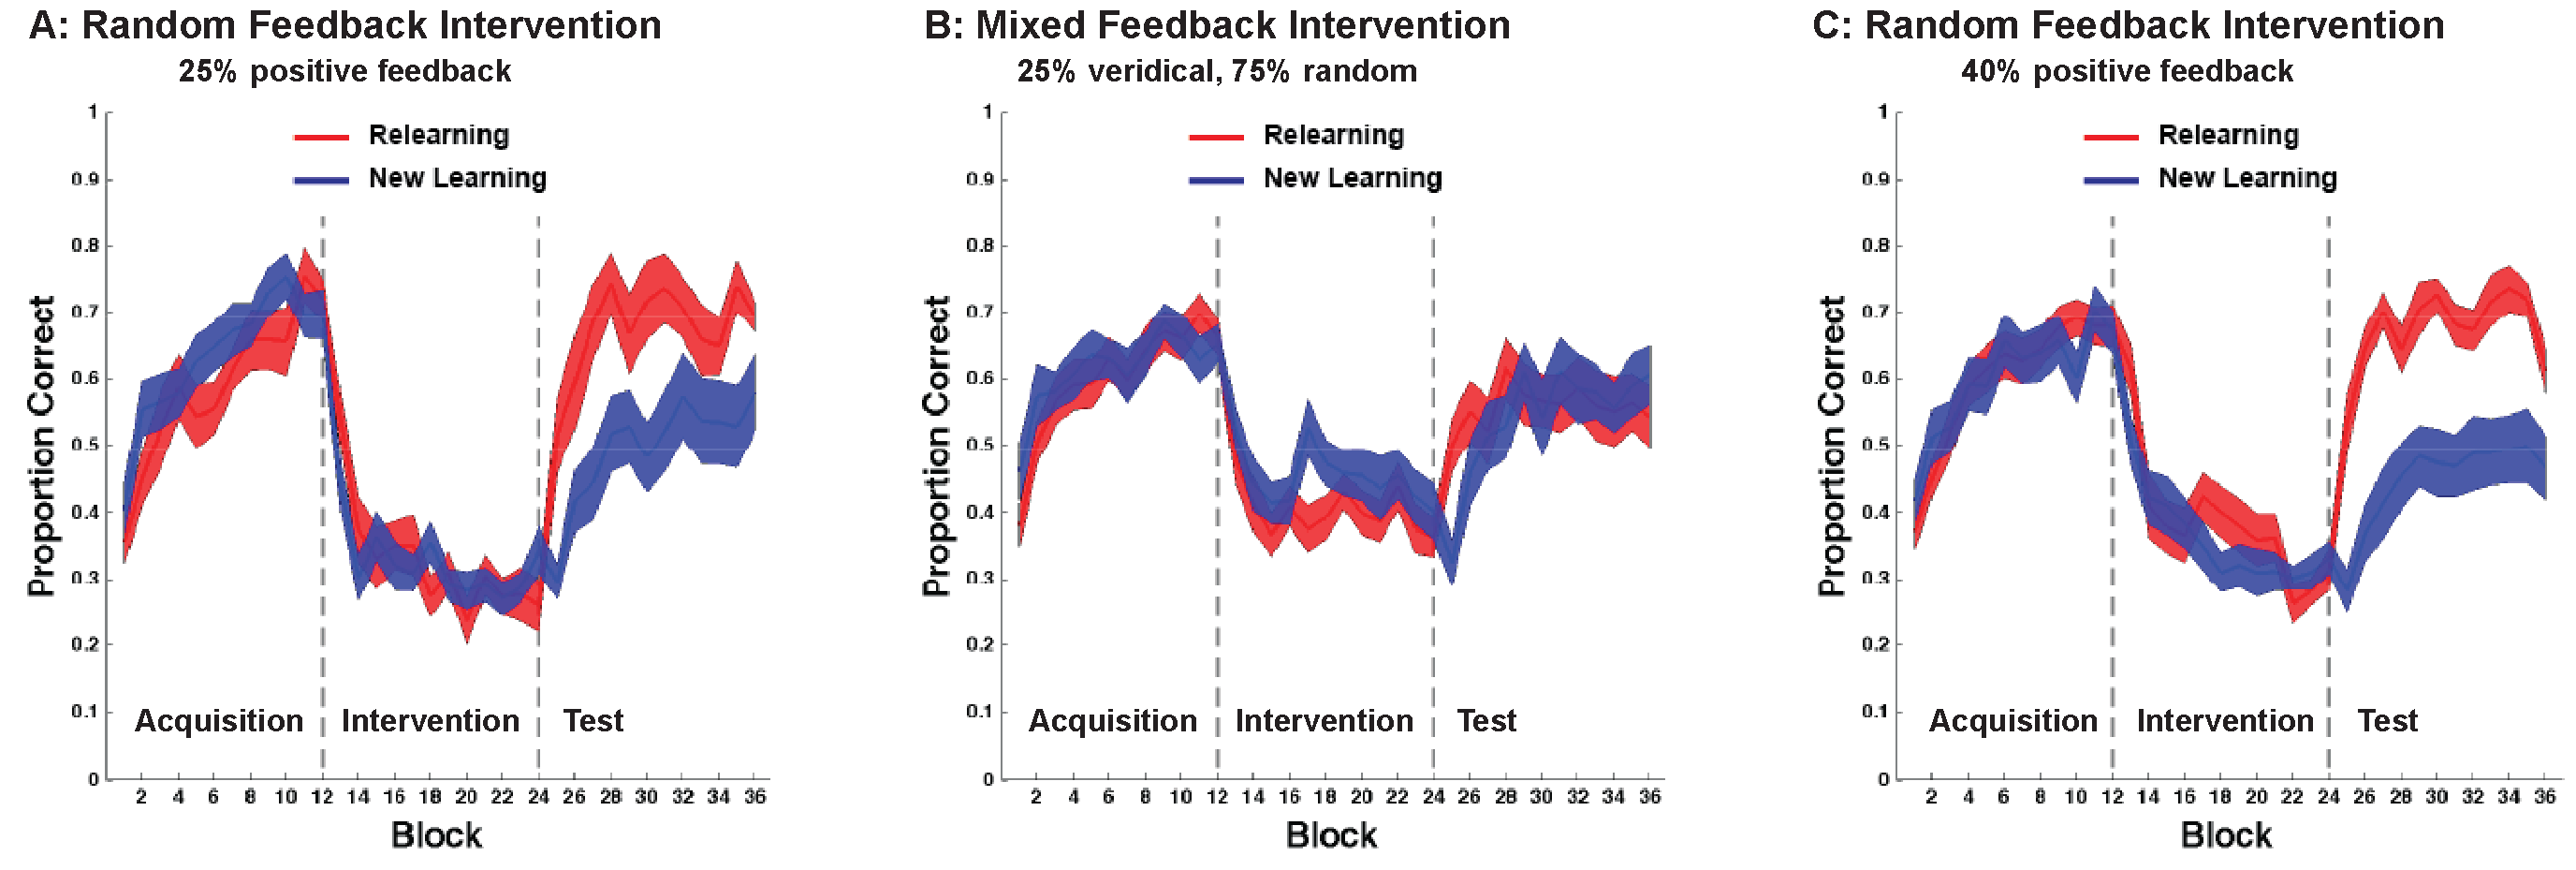
\includegraphics[width=1.0\textwidth]{../figures/fig_unlearning_results.pdf}
\caption{Crossley et al. (2013) behavioral results with different
  interventions. \textbf{A:} Random feedback intervention with 25\% positive
  feedback. Accuracy drops to near chance during intervention, but is reacquired
  faster than original learning in the Relearning condition (red). In contrast, a
  lasting interference is observed in the New Learning condition (blue). Both
  results are consistent with the hypothesis that initial learning was not
  overwritten by random feedback. \textbf{B:} Mixed feedback intervention.
  Accuracy drops during intervention -- though not to chance (i.e., 25\%) -- but
  subsequent learning proceeds at approximately the same rate and to the same
  extent as initial learning when either the original category-response mappings
  (red) or new category-response mappings (blue) are introduced. These results are
  consistent with the hypothesis that initial learning was overwritten during the
  intervention. \textbf{C:} Random feedback intervention with 40\% positive
  feedback. Results are qualitatively identical to random feedback intervention
  with 25\% positive feedback, implying that the mixed feedback results were
  driven by feedback contingency and not by positive feedback. }
  \label{fig:unlearning_data}
\end{figure}

\subsection*{The Present Study}
Crossley et al. (2013) hypothesized that the gate on procedural learning --- and
therefore the key to procedural modification --- is controlled by the degree of
feedback contingency, but we made no predictions about how feedback contingency
is estimated by the nervous system. This article begins addressing this question
-- by asking whether the estimation of feedback contingency depends on executive
function (e.g., prefrontal networks involved in working memory and executive
reasoning). Our rationale is as follows: If feedback contingency is estimated by
executive mechanisms, then increasing cognitive load during the intervention
phase (by requiring participants to simultaneously perform a dual task) should
impair the ability of participants to detect random feedback. This should in
turn cause the TANs gate to remain open, thereby allowing RF to modify the
procedural knowledge that was acquired during initial learning.

With this goal in mind, we performed an experiment that mimicked the design of
Crossley et al. (2013), except we added a concurrent numerical Stroop task
during key classification trials. Previous research suggests that this dual task
interferes with category learning that recruits executive function and
declarative memory much more than with category learning that recruits
procedural memory \cite{WaldronAshby2001, crossley2016declarative}, and that the
types of categories used here recruit procedural learning even when the
dual task is being performed \cite{crossley2016declarative}.

In conditions 1 -- 3, the first dual-task trial was 50 trials before the onset
of intervention, and continued for 100, 200, or 300 trials, respectively. In
Condition 4, the first dual-task trial was 50 trials after the onset of
intervention, and continued for 250 trials. Comparing conditions 1 through 3
allow us to look for a dose dependency. Condition 4 allows us to assess the
importance of disrupting the estimation of feedback contingency during the
transition from acquisition to intervention. Condition 5 was a control condition
in which no concurrent Stroop task was ever performed.

If feedback contingency estimation depends on executive function then two
behavioral markers are expected: (1) the dual task should slow the drop in
categorization accuracy that occurs with the onset of RF; and (2) reacquisition
of the original category learning should be slower in the dual task conditions
than in the no dual-task control.

\section*{Methods}
\subsection*{Design} There were four dual-task conditions (Condition 1 -- 4) and
one no dual-task control condition (Condition 5). The dual-task conditions
differed on two dimensions, (1) the number of trials on which the dual task was
applied, and (2) whether or not the onset of the dual task preceded the onset of
intervention.

\subsection*{Participants} 163 participants were recruited from the University
of Texas at Austin undergraduate population. There were 30 participants in
Condition 1, 34 participants in Condition 2, 32 participants in Condition 3, 33
participants in Condition 4, and 34 participants in Condition 5. After
exclusions (described in the next subsection), 119 participants were included in
the reported analyses. Of these, there were 23 in Condition 1, 26 in Condition
2, 22 in Condition 3, 21 in Condition 4, and 27 in Condition 5. All participants
completed the study and received course credit for their participation. All
participants had normal or corrected-to-normal vision.

\subsection*{Exclusions}
Of these 163 participants, 25 were excluded from the reported analyses for
failing to reach a an average accuracy of 40\% correct during the last 50 trials
of the acquisition phase (described below). An additional 19 were excluded for
failing to perform the concurrent numerical Stroop task with an average accuracy
greater than or equal to 80\%.

\subsection*{Stimuli and Categories} Stimuli were black lines that varied across
trials only in length (pixels) and orientation (degrees counterclockwise
rotation from horizontal). The stimuli are illustrated graphically in Figure 1,
and were identical to those used by Crossley et al. (2013).

\subsection{Procedure} Participants in all conditions were told that they were
to categorize lines on the basis of their length and orientation, that there
were four equally-likely categories, and that high levels of accuracy could be
achieved. The experiment included three phases: acquisition (300 trials),
intervention (400 trials), and reacquisition (150 trials). During acquisition
and reacquisition, feedback was based on the participant's response, whereas
feedback was random during the intervention. Participants were given no prior
instructions about the phases, and the transition from one phase to another
occurred without any warning to the participant.

At the start of each non-Stroop trial, a fixation point was displayed for 1
second and then the stimulus appeared. The stimulus remained on the screen until
the participant generated a response by pressing the ``Z'' key for category
``A'', the ``W'' key for category B, the ``/'' key for category C, or the ``P''
key for category D. Written instructions informed participants of the category
label to button mappings. An ``invalid key'' message was displayed if any other
button was pressed. The word ``Correct'' was presented for 1 second if the
response was correct or the word ``Wrong'' was presented for 1 second if the
response was incorrect (except during the intervention phase in which feedback
was completely random).

Stroop trials began with a fixation point that was displayed for 1 second. The
category stimulus and the Stroop stimuli (numbers flanking the category
stimulus) were displayed simultaneously. After 200 ms the Stroop stimuli were
replaced by white rectangles which remained on the screen until they made a
category response. Responses emitted before the Stroop stimuli were replaced by
white rectangles were not accepted. Feedback about the category response was
given immediately in the same fashion as on non-Stroop trials. The word
``value'' or ``size'' then appeared on the screen prompting participants to
indicate which side contained the numerically larger or the physically larger
number. Participants pressed the ``F'' key to choose the number on the left or
the ``J'' key to choose the number on the right. The word ``Correct'' was then
again presented for 1 second if the response to the Stroop task was correct or
the word ``Wrong'' was presented for 1 second if the response was incorrect. See
Figure 1 for example trials both including and excluding the Stroop component.
The Stroop task was included on trials 251-350 in condition 1, 251-450 in
condition 2, 251-550 in condition 3 and 350-600 in condition 4.

Participants were instructed to try their hardest on both task components but to
prioritize performance on the Stroop task. Both the category-learning task and
the Stroop task were explained to participants prior to beginning the
experiment, and on screen messages warned them when the Stroop component would
begin, and again when it would end. These messages read, ``You will now perform
both the categorization task and the paired numbers task simultaneously. Keep
trying your hardest!'' and ``You have now finished the section with the paired
numbers task. You will now be shown only the line categorization task. Keep
trying your hardest.'' 85\% of Stroop trials the numerically larger number was
physically smaller. The proportion of Stroop trials that prompted ``size'' or
``value'' was split 50/50. Accuracy on the numerical Stroop task was indicated
at the top of the screen when they received feedback regarding their performance
on the concurrent task on each trial. This score was displayed in green if it
was above 80\% and red if it was below 80\%. Note that when we refer to the
``dual-task'', we are referring to the Stroop task just described.

\subsection*{Statistical Analyses}
All t-tests comparing effects between conditions use the Welch-Satterthwaite
approximation to the degrees of freedom to account for violations of homogeneity
of variance.

\section*{Results}
\subsection*{Numerical Stroop Accuracy}
\begin{figure}[t]
\centering 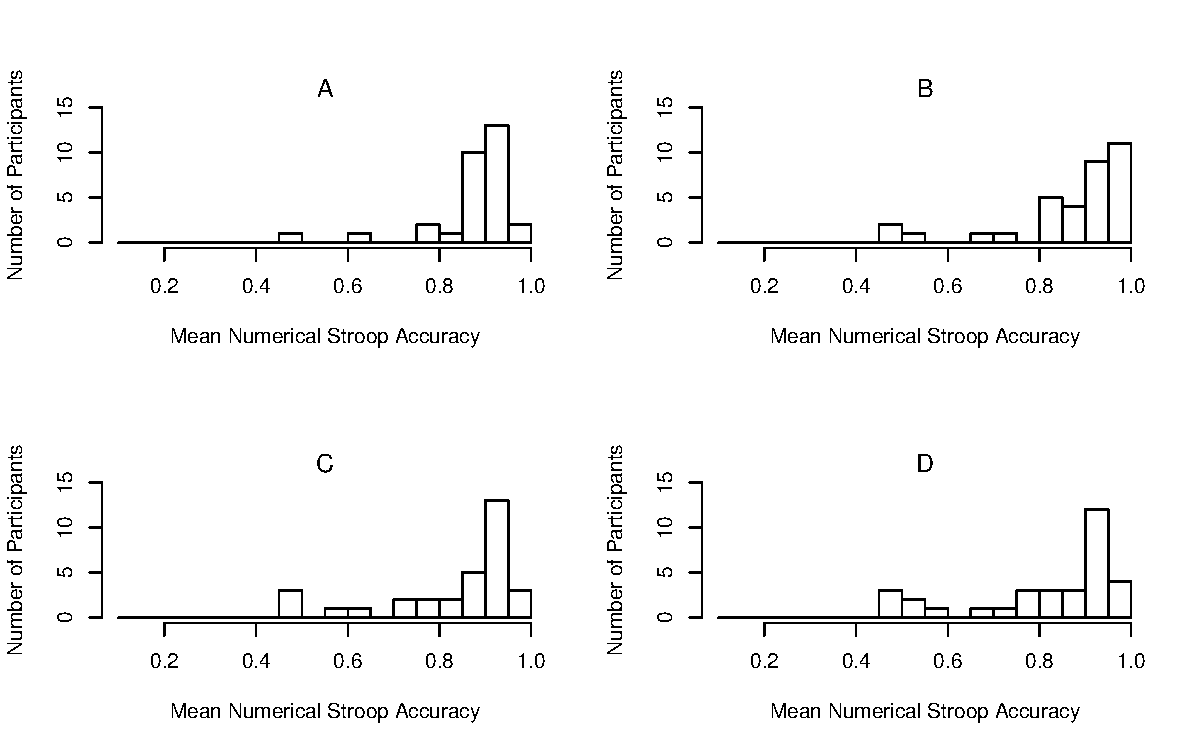
\includegraphics[width=1.0\textwidth]{../figures/fig_exc_dual.pdf}
    \caption{ Histograms showing distribution of mean Numerical Stroop accuracy
seperately for each condition. \textbf{A:} Condition 1. \textbf{B:} Condition 2.
\textbf{C:} Condition 3. \textbf{D:} Condition 4. }
    \label{fig:exc_dual}
\end{figure}

Figure \ref{fig:exc_dual} shows histograms characterizing mean dual-task
performance seperately for each condition. Overall, mean accuracy on the
dual-task was very good, with mean proportion correct at $0.88$ in Condition 1,
$0.87$ in Condition 2, $0.84$ in Condition 3, and $0.82$ in Condition 4.
Participants that failed to perform the dual-task with an average accuracy
greater than or equal to 80\% were excluded from further analyses (see the
``Exclusions'' section above).

\subsection*{Classification Accuracy}
\begin{figure}[t]
\centering 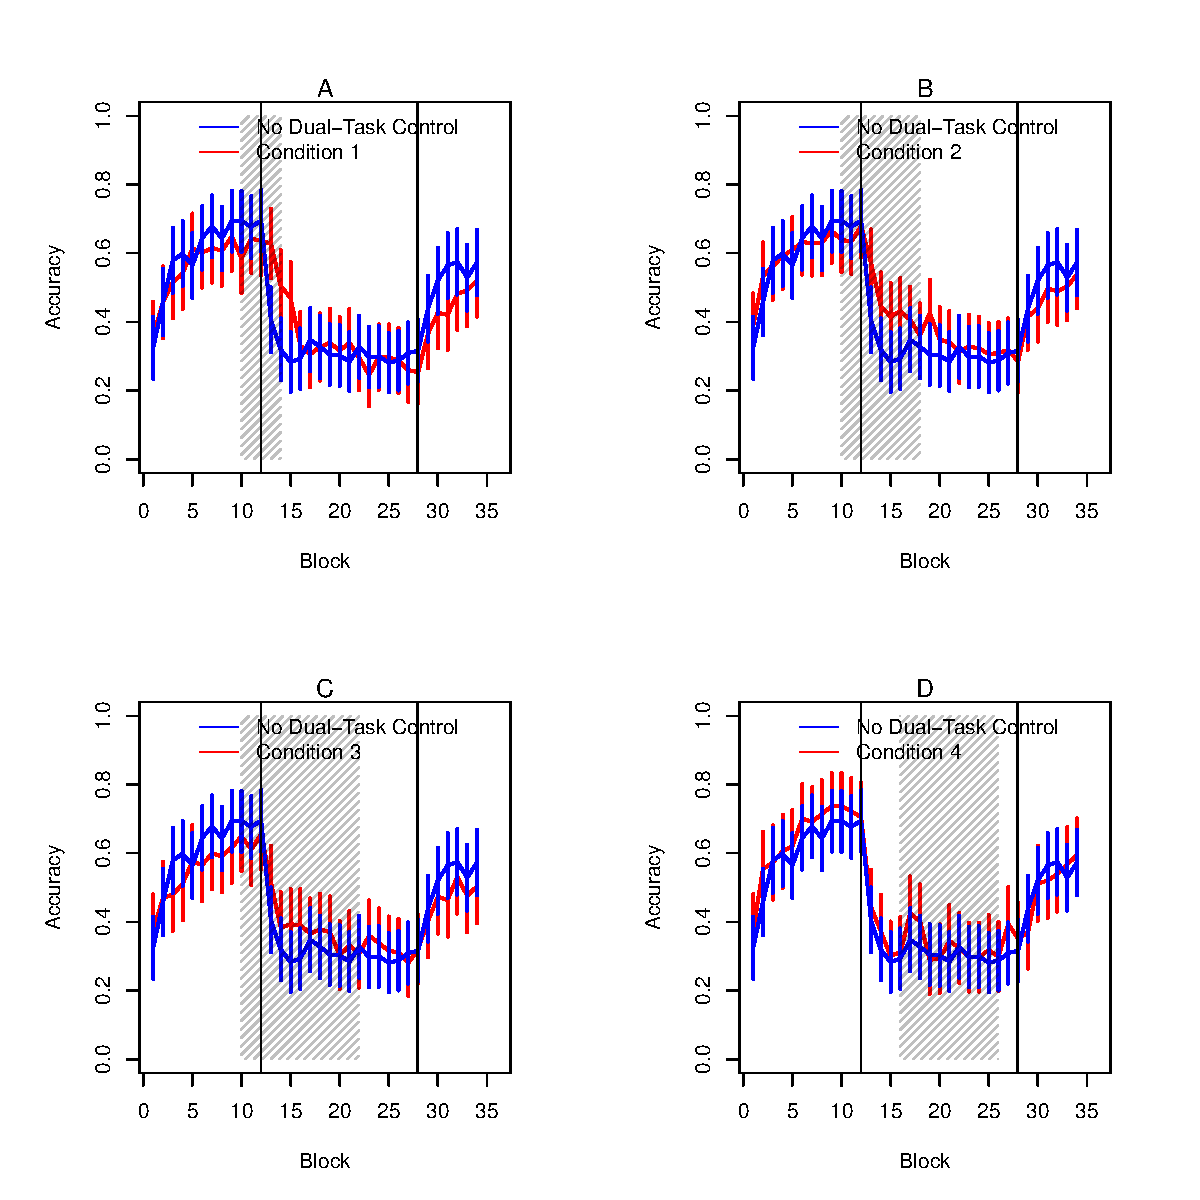
\includegraphics[width=1.0\textwidth]{../figures/fig_learning_curves.pdf}
\caption{ Mean accuracy per 25 trial block. The blue line in each panel is
  Condition 5 (no dual-task control). The hatch marks indicate dual-task trials.
  The key features are (1) dual-task slows the change in classification strategy
  (seen in this plot as ``accuracy'' decline), and (2) the dual-task conditions
  show less savings than the no dual-task control. There is no obvious
  dose-dependent effect of the dual task, nor is there an obvious difference
  between dual-task conditions.
  \textbf{A:} Condition 1 (dual-task applied on trial 251 through trial 350).
  \textbf{B:} Condition 2 (dual-task applied on trial 251 through trial 450).
  \textbf{C:} Condition 3 (dual-task applied on trial 251 through trial 550).
  \textbf{D:} Condition 4 (dual-task applied on trial 351 through trial 650).
  Error bars are SEM. }
  \label{fig:learning_curves}
\end{figure}

Figure \ref{fig:learning_curves} shows the mean accuracy in each block of 25
trials across the duration of the experiment. Recall that if feedback
contingency is estimated via executive mechanisms, then (1) dual-task trials
should slow the change in classification performance during intervention, and
(2) dual-task conditions should show reduced savings relative to the no
dual-task control. We see evidence for both features in our data.

\subsubsection*{Acquisition}
Conditions 1 -- 5 are identical for the first 250 trials (10 blocks) of
acquisition (before dual-task onset), and so we expect performance during these
blocks to be the same across conditions. However, Figure
\ref{fig:learning_curves} shows modest differences between some of the
conditions. A 5 Condition $\times$ 10 Block repeated-measures ANOVA revealed a
significant main effect of Condition $F(4,1180) = 8.29, p < 0.01, \Omega = 0.02$,
and a significant main effect of Block $F(1,1180) = 250.83, p < 0.01, \Omega =
0.17$, but no significant interaction $F(4,1180) = 1.95, p = 0.10, \Omega =
0.01$. Posthoc t-tests indicated that the main effect of Condition was driven by
Condition 1 being significantly less than Condition 4 [$t(39) = -2.26, p < 0.05,
d = 0.81$] and Condition 3 being significantly less than Condition 4 [$t(41) =
2.30, p < 0.05, d = 0.82$].


\subsubsection*{Intervention}
If the estimation of feedback contingency depends on  executive function,
then we expect change in performance during intervention to be slowed during the
simultaneous performance of the dual task. This is clearly seen in the first
four blocks of the intervention phase, and is supported by the results of a 5
condition $\times$ 4 block repeated-measures ANOVA. A significant effect of
Condition [$F(4,466) = 17.34, p < 0.001, \Omega = 0.11$] primarily reflected an
overall difference in intervention performance in dual-task conditions relative
to the no dual-task control. The effect of Block and the interaction between
Condition and Block were also significant [Block: $F(1,466) = 59.37, p < 0.001,
\Omega = 0.10$; Condition: $F(4,466) = 2.41, p < 0.05, \Omega = 0.02$].
The directional interpretation of the omnibus test is supported by several
planned comparisons on the overall mean accuracies during the first four blocks
of the intervention phase. First, early intervention accuracy in all dual-task
conditions in which the dual-task was introduced before the onset of the
intervention phase was significantly different from intervention accuracy in the no
dual-task control
[
condition 1 vs condition 5: $t(41) = 5.34, p < 0.01, d = 4.44$;
condition 2 vs condition 5: $t(47) = 4.99, p < 0.01, d = 3.61$;
condition 3 vs condition 5: $t(36) = 2.87, p < 0.05, d = 1.38$;
condition 4 vs condition 5: $t(31) = 0.88, p = 0.38, d = 0.14$ 
].

\subsubsection*{Savings}
\begin{figure}[t]
\centering 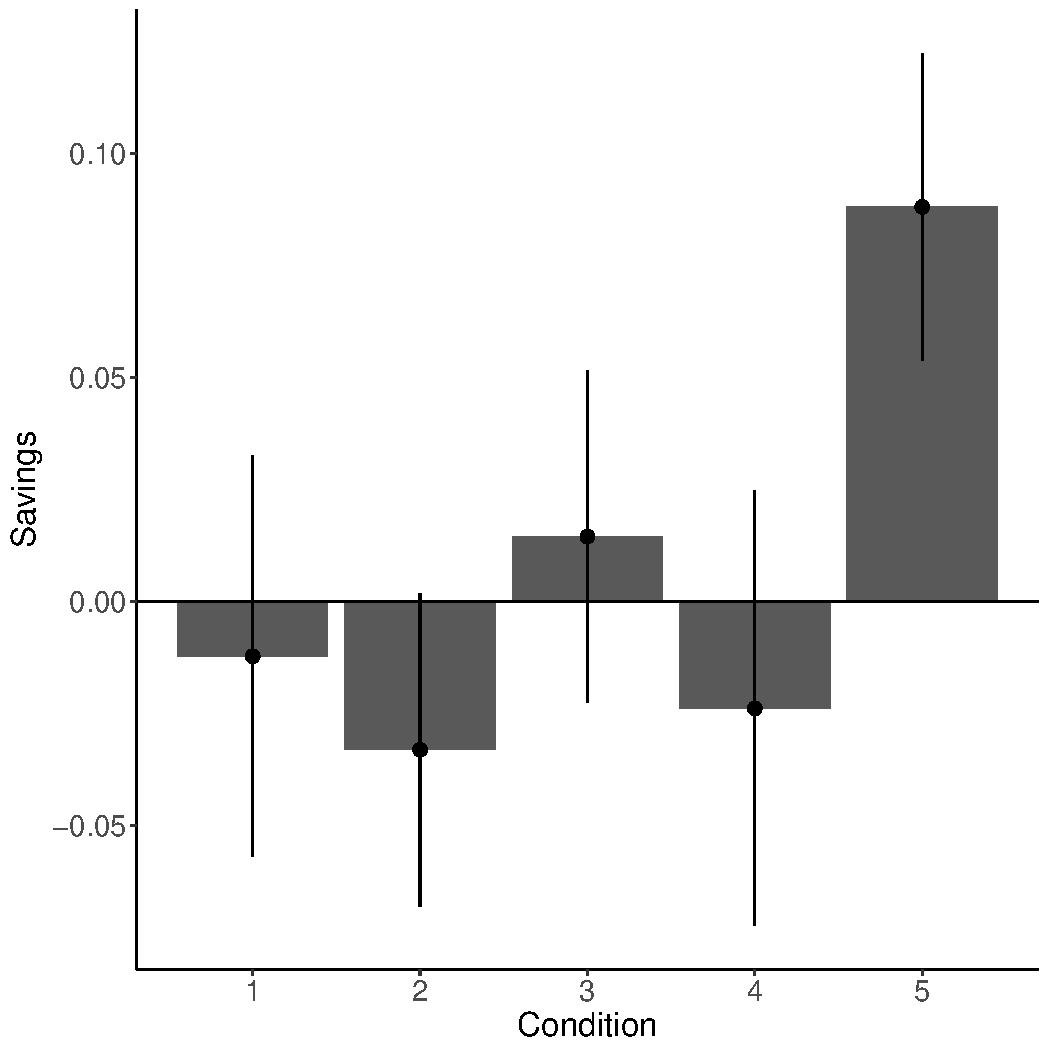
\includegraphics[width=1.0\textwidth]{../figures/fig_savings.pdf}
\caption{Savings (mean of the first 50 reacquisition trials - mean of the first
  50 acquisition trials) in all conditions of the present experiment.
  Error bars are SEM.}
  \label{fig:savings}
\end{figure}

If the computation of feedback contingency depends on executive function, then
we expect the dual-task conditions to exhibit less savings than the no dual-task
control -- that is, we expect reacquisition of the original categories to be
slower under dual-task conditions. This is apparent via visual inspection of
Figure \ref{fig:savings}, which shows the mean savings per condition.

There was no significant savings in any of the dual-task conditions [Condition
1: $t(22) = -0.27, p = 0.79, d = 0.02$; Condition 2: $t(25) = -0.95, p = 0.35, d
= 0.18$; Condition 3: $t(21) = 0.39, p = 0.70, d = 0.03$; Condition 4: $t(20) =
-0.49, p = 0.63, d = 0.05$; ], but there was significant savings in the no
dual-task control condition [Condition 5: $t(26) = 2.57, p < 0.05, d = 1.29$ ].

Moreover, the savings observed in Condition 5 was significantly greater than in
all dual-task conditions except Condition 3
[
Confition 1 < Condition 5: $t(43) = -1.78, p < 0.05, d = 0.48$;
Confition 2 < Condition 5: $t(51) = -2.47, p < 0.05, d = 0.86$;
Confition 3 < Condition 5: $t(45) = -1.45, p = 0.08, d = 0.31$;
Confition 4 < Condition 5: $t(38) = -1.88, p < 0.05, d = 0.58$
], and was significantly greater than the savings pooled across all dual-task
conditions [$t(26) = 2.57, p < 0.05, d = 1.29$].

Recall that our design was constructed to allow for an examination of
dose-dependency between conditions 1, 2, and 3. To answer this question, we
performed a 1-way ANOVA asking if savings is different between Conditions 1
through 3. There was no significant difference between these conditions
[$F(1,69) = 0.22, p = .64, \Omega = 0.003$], indicating that we did not observe
a dose-dependency.

We also designed our experiment to investigate the importance of placing the
dual-task on the transition from acquisition to intervention. Since Condition 4
is significantly greater than Condition 1 and 3, we can only examine this
question by comparing Condition 2 to Condition 4. A t-test revealed no
significant difference [$t(41) = .18, p = .86, d = 0.06$], indicating that we
found no evidence suggestion that the placement of the dual-task matters.

\section*{Discussion}
\subsection*{Summary}
Our results support our earlier conclusion \cite{crossley_erasing_2013} that
feedback contingency, defined as the correlation between response confidence and
feedback valence, may be key to controlling a gate that prevents or permits the
modification of procedural SR associations. To our knowledge, this article
reports results from the first behavioral experiments that investigate the
cognitive mechanisms that estimate feedback contingency. Specifically, our goal
was to determine whether executive function and declarative memory mechanisms
mediate contingency estimation. If they do, then a dual task that depends on
working memory and executive function should make it more difficult for
participants to recognize the sudden onset of random feedback. In our
experiments, behavioral signatures of this difficulty would include (1) a slowed
decrease in classification accuracy during intervention, and (2) decreased
savings in relearning relative to a no dual-task control. Our results were
consistent with both of these predictions.

Our design allowed us to ask not just whether contingency estimation relies on
executive function, but also whether the effects of disrupted contingency
estimation are dose dependent (i.e., whether effects increase with dual-task
exposure), and also whether it is important for the dual task to overlap with
the transition from acquisition to intervention. We found no evidence for either
of these possibilities.

% NOTE: consider removing this section
\subsection*{Category Learning as a Procedural Skill}
A natural question for readers unfamiliar with the category-learning literature
is whether our behavioral paradigm is a good choice for studying procedural
behaviors. In other words, how can a task with such simple motor demands (e.g.,
push a button) possibly recruit procedural networks that are strongly tied to
motor processes? In fact, the empirical evidence is strong that performance
improvements in the classification task used here are mediated via procedural
learning and memory. A large database of evidence suggests that humans have
multiple, qualitatively distinct category-learning systems \cite{AshbyCOVIS1998,
AshbyMaddox2005, EricksonKruschke1998}, and according to this view, procedural
memory is used to form many-to-one stimulus-to-response mappings (S-R
associations), whereas executive function and declarative memory are used to
apply rules and test explicit hypotheses about category membership.

The majority of this evidence comes from prior research with rule-based (RB) and
information-integration (II) category-learning tasks \cite{HelieRoederAshby2010,
NomuraEtAl2007, SotoEtAl2013, WaldschmidtAshby2011}. In RB tasks, the categories
can be learned via an explicit hypothesis-testing procedure
\cite{AshbyCOVIS1998}. In the simplest variant, only one dimension is relevant
(e.g., bar width), and the task is to discover this dimension and then map the
different dimensional values to the relevant categories. In II tasks, accuracy
is maximized only if information from two or more stimulus dimensions is
integrated perceptually at a pre-decisional stage \cite{AshbyGott1988}. In most
cases, the optimal strategy in II tasks is difficult or impossible to describe
verbally \cite{AshbyCOVIS1998}. Verbal rules may be (and sometimes are) applied,
but they lead to suboptimal performance. The task used here (and illustrated in
Figure 1) was an II category-learning task.

At least 25 different behavioral dissociations tie II learning to procedural
memory (and RB learning to executive function and declarative memory; for reviews, see
\citeNP{AshbyMaddox2005, AshbyMaddox2010, AshbyValentin2016a}). For example, one
behavioral signature of procedural learning is that because of its motor
component, switching the locations of the response keys interferes with
performance \cite{WillinghamButtonSwitch2000}. In agreement with this result,
switching the locations of the response keys interferes with II categorization
performance, even when the task only includes two categories\footnote{In
contrast, the same button switch does not interfere with RB performance in tasks
where the RB categories are created by simply rotating the II categories by
$45^\circ$} \cite{AshbyEllWaldron2003, MaddoxBohilIng2004, SpieringAshby2008}.

This hypothesis is further supported by a variety of investigations into the
neural underpinnings of successful II and RB learning. Specifically, success in
RB tasks depends on a broad neural network that includes the prefrontal cortex
(PFC), anterior cingulate, the head of the caudate nucleus, and medial temporal
lobe structures---regions that are also frequently associated with declarative
memory and executive attention \cite{BrownMarsden1988, FiloteoEtAl2007,
MuhammadWallisMiller2006, SegerCincotta2006}. Success in II tasks, on the other
hand, depends on regions that have been implicated in procedural memory,
including the striatum, premotor cortex, and the associated sensorimotor basal
ganglia loop \cite{AshbyEnnis2006, FiloteoMaddoxSalmonSong2005,
KnowltonMangelsSquire1996, NomuraEtAl2007}. This network is consistent with the
idea that S-R associations are built at cortical-striatal synapses via
dopamine-dependent reinforcement learning \cite{AshbyCrossley2011,
HoukAdamsBarto1995, joel_actorcritic_2002}.

\subsection*{Therapeutic Relevance}
The old adage of ``it's like riding a bike'' is a surprisingly accurate
description of procedural knowledge, reflecting its remarkable retention over
years without practice. Paradigms designed to study procedural learning in the
lab have echoed this adage, reporting savings in learning up to a year after
training \cite{Romano2010, turner_long-term_2012}. However, the stability of
procedural memory comes at the cost of remarkable inflexibility. For example,
changing any stimulus or response parameter that was present during training can
prove catastrophic to performance \cite{Rozanov_2010, Dienes_1997}. While
resilience and inflexibility are desirable traits when a useful skill has been
sufficiently learned, they can also lead to persistent maladaptive behaviors
that have serious negative consequences, and in some cases may prove detrimental
to a person's health (e.g., drug abuse). Unfortunately, neither the potential
for modification of procedural knowledge, nor a method to do so, are well
understood.

Our previous research identified the interplay between striatal cholinergic
interneurons and the midbrain dopamine system in controlling the eligibility of
procedural knowledge for modification \cite{AshbyCrossley2011,
crossley_erasing_2013}. Directly targeting this network for improved
interventions is unfortunately challenging, due to the difficulty of
manipulating and measuring subcortical networks. Here, insofar as increasing
cognitive load via a dual-task taps into prefrontal networks, we looked for more
easily accessible cortical substrates that may control the striatal mechanism.
Our results indicate that prefrontal networks likely do play an important role
in controlling the estimation of feedback contingency, and therefore may provide
an accessible cortical target for electrical or magnetic intervention.

\bibliography{bibs/cdl,bibs/cdl_2,bibs/crossley}

\end{document}
